\documentclass[11pt]{article}
\usepackage[margin=0.78in]{geometry}
\usepackage{booktabs}
\usepackage{array}
\usepackage{float}
\usepackage{amsmath}
\usepackage[table]{xcolor}
\usepackage[hidelinks]{hyperref}
\usepackage[numbers]{natbib}
\usepackage{microtype}
\usepackage{pgfplots}
\pgfplotsset{compat=1.16}

\definecolor{accent}{HTML}{2F6F7E}
\definecolor{cdk}{HTML}{0072B2}
\definecolor{tyk}{HTML}{D55E00}
\definecolor{jnk}{HTML}{009E73}
\definecolor{pth}{HTML}{CC79A7}
\definecolor{highlightbg}{HTML}{EAF4F6}
\definecolor{nessobg}{HTML}{E8F5E9}
\definecolor{boltzbg}{HTML}{E8F0FA}
\definecolor{diffbg}{HTML}{FFF2CC}
\hypersetup{colorlinks=true,linkcolor=accent,citecolor=accent,urlcolor=accent}
\setlength{\parindent}{0pt}
\setlength{\parskip}{0.48em}

\title{\textbf{Week of August 17, 2026}\\
Boltz-2, Nesso-1, FlashBind, and an FEP+ four-kinase reproduction}
\author{Yusheng Cai}
\date{August 17--23, 2026}

\begin{document}
\maketitle
\begin{center}
  \small GitHub folder for this week:
  \href{https://github.com/Yusheng-cai/BindingAffinityPredictor/tree/main/weeks/2026-W34}%
       {\texttt{weeks/2026-W34}}
\end{center}

\section*{Executive summary}

This report compares three released protein--ligand affinity workflows.
Boltz-2 cofolds an atom-resolved complex and predicts affinity; Nesso-1
predicts affinity without coordinate diffusion or an MSA; and, in this
benchmark, FlashBind scores a FABind+-predicted ligand pose in an experimental
PDB protein structure
\citep{passaro2025boltz2,shenoy2026nesso1,jiang2026flashbind}.

I ran all three models on the public 87-compound, four-kinase benchmark and
compared predicted scores with experimental potency within each kinase. The
weighted Pearson correlations below closely reproduce the paper values. I
also evaluated the predicted protein-ligand structure from Boltz-2 and the released FABind+ against the 16 experimentally available bound structures.

\begin{center}
\setlength{\fboxsep}{9pt}
\fcolorbox{accent}{highlightbg}{%
\parbox{0.91\textwidth}{
\centering
\textbf{\color{accent}\large Headline results}\\[0.45em]
\textbf{Affinity ranking: 87 compounds}\\[0.25em]
\begin{tabular}{@{}lccc@{}}
\toprule
 & \textbf{Weighted Pearson $r$} & \textbf{95\% interval} & \textbf{Paper reference} \\
\midrule
Nesso-1 & \textbf{0.807} & 0.731--0.873 & 0.80 \\
Boltz-2 MSA-1024 & \textbf{0.627} & 0.484--0.744 & 0.66 \\
FlashBind, released poses & \textbf{0.533} & 0.382--0.669 & 0.53 \\
\bottomrule
\end{tabular}\\[0.65em]
\textbf{Structure recovery: median RMSD over 16 cocrystals (\AA)}\\[0.25em]
{\small
\begin{tabular}{@{}>{\raggedright\arraybackslash}p{2.35in}>{\centering\arraybackslash}p{1.55in}>{\centering\arraybackslash}p{1.95in}@{}}
\toprule
 & \shortstack{\textbf{Boltz-2}\\predicted protein\\+ ligand}
 & \shortstack{\textbf{FlashBind}\\experimental PDB protein\\+ FABind+-predicted\\ligand position} \\
\midrule
Global protein C$\alpha$, fitted & 1.231 & 0.272 \\
Pocket protein C$\alpha$, fitted & 0.400 & 0.208 \\
Ligand heavy atoms after pocket fit & \textbf{0.898} & \textbf{0.634} \\
\bottomrule
\end{tabular}
}
}}
\end{center}

\section{Benchmark}
Each target defines one separate medicinal-chemistry series: the protein is
held fixed while
the ligand is changed. The four targets are cyclin-dependent kinase 2 (CDK2),
tyrosine kinase 2 (TYK2), c-Jun N-terminal kinase 1 (JNK1), and p38$\alpha$
mitogen-activated protein kinase. All four are protein kinases, but they are
different proteins with different ligand series and different biochemical
assays.

\begin{table}[H]
\centering
\small
\begin{tabular}{@{}>{\raggedright\arraybackslash}p{1.70in}r>{\raggedright\arraybackslash}p{2.25in}>{\raggedright\arraybackslash}p{0.72in}c@{}}
\toprule
Target / assay series & Ligands ($N$) & Protein construct input & Endpoint & \shortstack{Reference\\PDB} \\
\midrule
CDK2 (cyclin-dependent kinase 2) & 16 & CDK2, 303 aa; cyclin A2, 258 aa & IC50 & 1H1Q \\
TYK2 (tyrosine kinase 2) & 16 & TYK2, 302 aa & Ki & 4GIH \\
JNK1 (c-Jun N-terminal kinase 1) & 21 & JNK1, 370 aa; JIP1 peptide, 11 aa & IC50 & 2GMX \\
p38$\alpha$ (MAPK14) & 34 & p38 kinase, 372 aa & IC50 & 3FLY \\
\bottomrule
\end{tabular}
\caption{Frozen benchmark composition.}
\end{table}

\textbf{Experimental endpoint.} This is the laboratory measurement used as
the benchmark's ground-truth label. IC50 is the concentration that produces
50\% inhibition under a particular assay protocol. Ki is an inhibition
constant inferred through an enzyme-kinetic model. Smaller IC50 or Ki means
stronger apparent inhibition. These endpoints are related but not
interchangeable, and neither should automatically be called a binding free
energy. Source values in nM or $\mu$M were converted to $\mu$M and then to
$\log_{10}(\mathrm{value}/\mu\mathrm{M})$ before comparison. CDK2, JNK1, and
p38 use IC50 labels; TYK2 uses Ki labels.

%Thus, for the CDK2 row, the calculation asks a concrete ranking question:
%given the same CDK2--cyclin A2 protein construct and 16 different ligands, does
%the ordering of Nesso's 16 predicted affinity scores agree with the ordering
%of the 16 experimental IC50 measurements? Pearson, Spearman, and Kendall
%statistics answer that question for CDK2. The procedure is repeated separately
%for TYK2, JNK1, and p38 before the four target-level results are aggregated.

%I took the protein sequences from the deposited RCSB entities. I retained
%cyclin A2 for CDK2 and the JIP1 peptide for JNK1 because those partners are present in
%the curated benchmark complexes. Ligands were represented by canonical,
%stereochemically explicit SMILES; all have %formal charge zero. Nesso and Boltz
%received no crystallographic pose, template, pocket annotation, hotspot, or
%experimental label. FlashBind received the authors' fixed protein structures
%and FABind+-predicted ligand poses; its label file was not used during
%inference.

\section{Model description: Boltz-2, Nesso-1, and FlashBind}

\subsection{Boltz-2: cofold and score}

Boltz-2 performs two related tasks: it predicts how biomolecules fit together
in three dimensions, and it estimates binding affinity. For a protein--ligand
calculation, we provide the protein sequence, the ligand chemistry, and an MSA.


Boltz-2 considers the protein and ligand together. It begins with a noisy
arrangement of their atoms and repeatedly adjusts the coordinates until it
produces a plausible three-dimensional protein--ligand complex. Because this procedure involves random sampling,
the model can generate more than one candidate structure.

The public Boltz-2 software returns the predicted atomic coordinates and
scores describing its confidence in the structure. For a protein--ligand
pair, it also reports a probability that the ligand binds and a continuous
affinity score that can be used to rank compounds \citep{passaro2025boltz2}.
These affinity outputs are learned from experimental assay data. They are not
direct alchemical calculations of an equilibrium $\Delta G_\mathrm{bind}$.

\subsection{Nesso-1: predict affinity without coordinate diffusion}

Nesso-1 follows a different affinity workflow. It does not run the
atom-coordinate diffusion decoder used by Boltz-2, and it supplies protein
context through pretrained ESM-2 embeddings instead of an MSA.

The Nesso paper reports more than a tenfold inference speed-up over Boltz-2,
and more than twentyfold on some larger targets, while matching or exceeding
Boltz-2 on its evaluated affinity benchmarks \citep{shenoy2026nesso1}. Nesso
does not return the atom-resolved complex produced by Boltz-2, so the two
models serve different structural needs. For this project, I compare their
released affinity outputs on identical protein and ligand inputs. Neither
affinity head is a molecular simulation or a direct calculation of
$\Delta G_{\mathrm{bind}}$; both are learned from experimental potency and
affinity labels.

\subsection{FlashBind: dock then score}

At the user-facing level, FlashBind can begin with a protein sequence and a
ligand SMILES. Internally, however, the sequence must first be resolved to a
three-dimensional receptor. The released preprocessing searches for an
experimental or predicted structure and can fall back to a structure
predictor when one is unavailable. FABind+ then identifies a candidate pocket
and places the ligand in that region \citep{jiang2026flashbind}.

Around this proposed pose, FlashBind constructs a local protein--ligand graph
and processes it with an E(3)-equivariant graph neural network. Consequently,
rotating or translating the complete coordinate system does not arbitrarily
change the prediction. Separate output heads can return a binary activity
probability or a continuous assay-derived affinity score. As with the other
models, this continuous score is not a thermodynamic calculation of
$\Delta G_{\mathrm{bind}}$.

This modularity separates pose generation from affinity scoring, which makes
large-library screening more practical:
\[
 \text{receptor conformation}
 \longrightarrow \text{pocket selection}
 \longrightarrow \text{docked pose}
 \longrightarrow \text{binding score}.
\]


\begin{center}
\setlength{\fboxsep}{8pt}
\fcolorbox{accent}{highlightbg}{\parbox{0.91\textwidth}{
\centering
\textbf{\color{accent}\large Model workflows at a glance}\\[0.6em]
\textbf{Boltz-2:} sequence + ligand + MSA
$\rightarrow$ joint trunk + atom diffusion
$\rightarrow$ atom-resolved complex + affinity\\[0.5em]
\textbf{Nesso-1:} sequence + ligand
$\rightarrow$ ESM-2 + pair trunk + predicted pocket
$\rightarrow$ affinity, without a final Cartesian complex\\[0.5em]
\textbf{FlashBind:} 3D protein structure + ligand
$\rightarrow$ FABind+ pocket and pose
$\rightarrow$ local EGNN score}}
\end{center}

\section{Benchmark calculation overview}

I evaluated the released versions of all three models on the same set
of 87 protein--ligand pairs.

\subsection{Nesso-1}

I supplied Nesso-1 with the protein sequence and ligand chemistry for each
pair. It inferred an interaction region and returned continuous affinity
scores without generating a final three-dimensional complex. All 87 pairs
completed successfully \citep{shenoy2026nesso1}.

\subsection{Boltz-2}

I supplied Boltz-2 with the same protein sequences and ligand chemistry, plus
a sequence MSA generated once for each unique protein chain. Boltz-2 produced
a sampled atom-resolved complex together with affinity outputs. Because the
complete MSAs exceeded the memory of the local 10~GiB GPU, I used the model's
documented 1,024-row MSA subsampling option for every pair. All 87 structure
and affinity calculations completed \citep{passaro2025boltz2}.

\subsection{FlashBind}

For FlashBind, I used the authors' released benchmark inputs: an experimental
PDB protein structure and a FABind+-predicted ligand pose for each pair,
together with their precomputed molecular representations. I reran the two
released affinity scorers and averaged their continuous outputs. I did not
rerun the upstream FABind+ pose generation, so this calculation evaluates the
released scoring stage rather than the complete docking-to-scoring pipeline.
All 87 pairs completed \citep{jiang2026flashbind}.

\section{Metric: affinity and structure}


\textbf{Affinity metrics} use all 87 compounds and test agreement between model
scores and experimental potency labels. The \textbf{structure metrics} use
only the 16 pairs which have experimentally available crystal structures and compare Boltz-2 with
the FlashBind/FABind+ poses.

\subsection{Affinity-ranking metrics on 87 compounds}

I calculated the primary statistic in two stages:
\[
 r_t = \operatorname{Pearson}\!\left(y_{t,i},\hat y_{t,i}\right),
 \qquad
 \bar r = \frac{\sum_t n_t r_t}{\sum_t n_t}.
\]
Thus, the comparison asks whether each model ranks compounds correctly
\emph{within} each kinase series and then averages the target-level statistics
using the compound counts. Spearman $\rho$ and Kendall $\tau$ provide
complementary rank-based comparisons.

\subsection{Comparison with experimental structures}

I identified 16 exact
FEP+4 ligand--target identities with available experimental crystal structures and compare FlashBind/FABind+ with Boltz-2.

For each pair, I defined the
experimental protein binding pocket as residues having any heavy atom within 5~\AA{} of the ligand. I then fitted the predicted structure to experimental pocket using only
matched protein C$\alpha$ atoms. I held that transform fixed while applying it
to the predicted ligand and calculated
\[
  \mathrm{RMSD}_{\mathrm{pose}}
  = \min_{\pi\in\mathcal{M}}
  \sqrt{\frac{1}{N}\sum_{i=1}^{N}
  \left\|R\mathbf{x}_i+\mathbf{t}-\mathbf{x}^{\mathrm{ref}}_{\pi(i)}\right\|^2},
\]
where $R$ and $\mathbf{t}$ come only from the protein fit and
$\mathcal{M}$ contains complete bond-order- and chirality-compatible atom
mappings. The minimum over $\mathcal{M}$ corrects for chemically equivalent
atom permutations.

\section{Results}

\begin{table}[H]
\centering
\small
\begin{tabular}{lrrr}
\toprule
Target & Pearson $r$ & Spearman $\rho$ & Kendall $\tau$ \\
\midrule
CDK2 & 0.748 & 0.759 & 0.550 \\
TYK2 & 0.917 & 0.921 & 0.767 \\
JNK1 & 0.666 & 0.667 & 0.482 \\
p38  & 0.869 & 0.894 & 0.723 \\
\midrule
\rowcolor{nessobg}
Compound-weighted & \textbf{0.807} & \textbf{0.819} & \textbf{0.641} \\
\bottomrule
\end{tabular}
\caption{Nesso-1 released-checkpoint reproduction. The paper reports a
compound-weighted Pearson correlation of 0.80 on this benchmark.}
\end{table}

\begin{table}[H]
\centering
\small
\begin{tabular}{lrrr}
\toprule
Target & Pearson $r$ & Spearman $\rho$ & Kendall $\tau$ \\
\midrule
CDK2 & 0.831 & 0.865 & 0.667 \\
TYK2 & 0.807 & 0.779 & 0.617 \\
JNK1 & 0.758 & 0.805 & 0.616 \\
p38  & 0.364 & 0.433 & 0.287 \\
\midrule
\rowcolor{boltzbg}
Compound-weighted & \textbf{0.627} & \textbf{0.666} & \textbf{0.497} \\
\bottomrule
\end{tabular}
\caption{Boltz-2 MSA-1024 released-checkpoint reproduction. The paper
references are weighted Pearson $r=0.66$ and Kendall $\tau=0.48$; the present
values are 0.627 and 0.497.}
\end{table}

\begin{table}[H]
\centering
\small
\begin{tabular}{lrrr}
\toprule
Target & Pearson $r$ & Spearman $\rho$ & Kendall $\tau$ \\
\midrule
CDK2 & 0.612 & 0.641 & 0.433 \\
TYK2 & 0.134 & 0.147 & 0.083 \\
JNK1 & 0.546 & 0.578 & 0.425 \\
p38  & 0.677 & 0.591 & 0.413 \\
\midrule
\rowcolor{highlightbg}
Compound-weighted & \textbf{0.533} & \textbf{0.515} & \textbf{0.359} \\
\bottomrule
\end{tabular}
\caption{FlashBind two-checkpoint ensemble using the authors' released
FABind+ poses. The reported references are weighted Pearson $r=0.53$ and
Kendall $\tau=0.38$; the present values are 0.533 and 0.359.}
\end{table}

\begin{figure}[H]
\centering
\begin{tikzpicture}
\begin{axis}[
  width=0.75\textwidth,
  height=0.49\textwidth,
  xlabel={Experimental potency within-target $z$ score},
  ylabel={Nesso-1 affinity within-target $z$ score},
  xmin=-2.8,xmax=2.8,ymin=-2.8,ymax=2.8,
  axis lines=left,
  grid=major,
  legend style={at={(0.02,0.98)},anchor=north west,draw=none,fill=white},
]
\addplot[black,dashed,domain=-2.8:2.8] {x};
\addlegendentry{identity}
\addplot[only marks,mark=*,cdk] table[x=observed_z,y=predicted_z,col sep=comma]
  {figures/nesso1_cdk2.csv};
\addlegendentry{CDK2}
\addplot[only marks,mark=square*,tyk] table[x=observed_z,y=predicted_z,col sep=comma]
  {figures/nesso1_tyk2.csv};
\addlegendentry{TYK2}
\addplot[only marks,mark=triangle*,jnk] table[x=observed_z,y=predicted_z,col sep=comma]
  {figures/nesso1_jnk1.csv};
\addlegendentry{JNK1}
\addplot[only marks,mark=diamond*,pth] table[x=observed_z,y=predicted_z,col sep=comma]
  {figures/nesso1_p38.csv};
\addlegendentry{p38}
\end{axis}
\end{tikzpicture}
\caption{Within-target standardized experimental and predicted potency. Lower
values correspond to stronger binding on both axes. Standardization removes
target-specific offsets and scale differences for visualization only; metrics
were computed from the unstandardized values.}
\end{figure}

\begin{figure}[H]
\centering
\begin{tikzpicture}
\begin{axis}[
  width=0.75\textwidth,
  height=0.49\textwidth,
  xlabel={Experimental potency within-target $z$ score},
  ylabel={Boltz-2 affinity within-target $z$ score},
  xmin=-2.8,xmax=2.8,ymin=-2.8,ymax=2.8,
  axis lines=left,
  grid=major,
  legend style={at={(0.02,0.98)},anchor=north west,draw=none,fill=white},
]
\addplot[black,dashed,domain=-2.8:2.8] {x};
\addlegendentry{identity}
\addplot[only marks,mark=*,cdk] table[x=observed_z,y=predicted_z,col sep=comma]
  {figures/boltz2_msa1024_cdk2.csv};
\addlegendentry{CDK2}
\addplot[only marks,mark=square*,tyk] table[x=observed_z,y=predicted_z,col sep=comma]
  {figures/boltz2_msa1024_tyk2.csv};
\addlegendentry{TYK2}
\addplot[only marks,mark=triangle*,jnk] table[x=observed_z,y=predicted_z,col sep=comma]
  {figures/boltz2_msa1024_jnk1.csv};
\addlegendentry{JNK1}
\addplot[only marks,mark=diamond*,pth] table[x=observed_z,y=predicted_z,col sep=comma]
  {figures/boltz2_msa1024_p38.csv};
\addlegendentry{p38}
\end{axis}
\end{tikzpicture}
\caption{Boltz-2 MSA-1024 standardized scores. The dispersed p38 series is
the main target-level departure from Nesso-1 and from the other Boltz targets.}
\end{figure}

\begin{figure}[H]
\centering
\begin{tikzpicture}
\begin{axis}[
  width=0.75\textwidth,
  height=0.49\textwidth,
  xlabel={Experimental potency within-target $z$ score},
  ylabel={FlashBind affinity within-target $z$ score},
  xmin=-2.8,xmax=2.8,ymin=-2.8,ymax=2.8,
  axis lines=left,
  grid=major,
  legend style={at={(0.02,0.98)},anchor=north west,draw=none,fill=white},
]
\addplot[black,dashed,domain=-2.8:2.8] {x};
\addlegendentry{identity}
\addplot[only marks,mark=*,cdk] table[x=observed_z,y=predicted_z,col sep=comma]
  {figures/flashbind_cdk2.csv};
\addlegendentry{CDK2}
\addplot[only marks,mark=square*,tyk] table[x=observed_z,y=predicted_z,col sep=comma]
  {figures/flashbind_tyk2.csv};
\addlegendentry{TYK2}
\addplot[only marks,mark=triangle*,jnk] table[x=observed_z,y=predicted_z,col sep=comma]
  {figures/flashbind_jnk1.csv};
\addlegendentry{JNK1}
\addplot[only marks,mark=diamond*,pth] table[x=observed_z,y=predicted_z,col sep=comma]
  {figures/flashbind_p38.csv};
\addlegendentry{p38}
\end{axis}
\end{tikzpicture}
\caption{FlashBind standardized scores from the released FABind+ poses. TYK2
is the clear weak target, whereas the other three series retain positive
within-target ranking relationships.}
\end{figure}

I obtained an aggregate Pearson result of $0.807$ for Nesso (95\% interval
$0.731$--$0.873$), which agrees closely with the reported $0.80$. 

For Boltz,
I obtained $0.627$ (interval $0.484$--$0.744$), which is 0.033 below the
paper reference of $0.66$; its Kendall result of 0.497 is 0.017 above the
paper reference of 0.48.

For FlashBind I obtained weighted Pearson $r=0.533$ (95\% interval
$0.382$--$0.669$), essentially identical to the reported $0.53$. The weighted
Kendall value was $0.359$, 0.021 below the reported $0.38$. Unfortunately, this is not independent
validation as the authors supplied the FABind+ poses and representations used by
their own scoring benchmark.

\begin{table}[H]
\centering
\small
\begin{tabular}{lrrr}
\toprule
Statistic & Nesso-1 & \shortstack{Boltz-2\\MSA-1024} & FlashBind \\
\midrule
\rowcolor{highlightbg}
Pearson $r$ & \textbf{0.807} & \textbf{0.627} & \textbf{0.533} \\
Spearman $\rho$ & 0.819 & 0.666 & 0.515 \\
Kendall $\tau$ & 0.641 & 0.497 & 0.359 \\
\bottomrule
\end{tabular}
\caption{Full matched comparison across the 87-compound benchmark. Each entry
is the compound-count-weighted mean of the corresponding within-target
statistic.}
\end{table}

\begin{figure}[H]
\centering
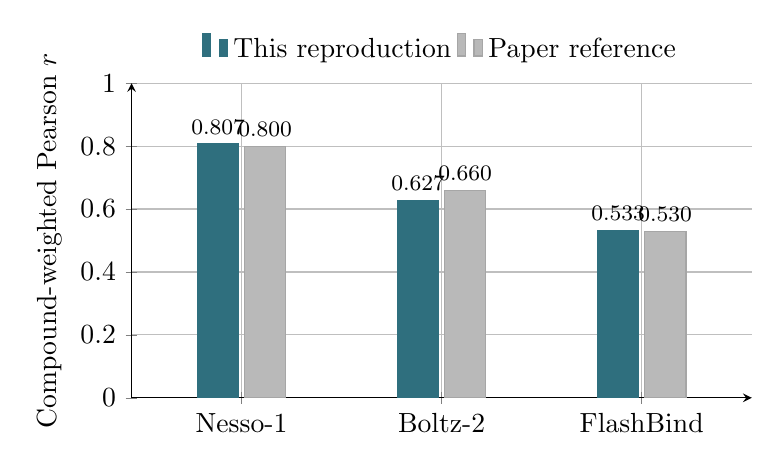
\begin{tikzpicture}
\begin{axis}[
  ybar,
  width=0.78\textwidth,
  height=0.46\textwidth,
  bar width=15pt,
  ymin=0,ymax=1.0,
  ylabel={Compound-weighted Pearson $r$},
  xmin=-0.55,xmax=2.55,
  xtick={0,1,2},
  xticklabels={Nesso-1,Boltz-2,FlashBind},
  axis lines=left,
  grid=major,
  nodes near coords={\pgfmathprintnumber[fixed,precision=3,fixed zerofill]{\pgfplotspointmeta}},
  nodes near coords style={font=\footnotesize},
  legend style={at={(0.5,1.03)},anchor=south,legend columns=2,draw=none},
]
\addplot[fill=accent,draw=accent] coordinates
  {(0,0.807) (1,0.627) (2,0.533)};
\addlegendentry{This reproduction}
\addplot[fill=gray!55,draw=gray!70] coordinates
  {(0,0.800) (1,0.660) (2,0.530)};
\addlegendentry{Paper reference}
\end{axis}
\end{tikzpicture}
\caption{Weighted within-target Pearson correlations from this reproduction
and the corresponding paper reference values. The reproduced values differ
from the references by $+0.007$ for Nesso-1, $-0.033$ for Boltz-2, and
$+0.003$ for FlashBind. Bars show point estimates; the bootstrap intervals
are reported in the text and executive-summary table.}
\end{figure}

There is, however, a large difference within the targets: Boltz is better on
CDK2 and JNK1,
Nesso is better on TYK2, and p38 supplies the largest Nesso advantage
($r=0.869$ versus $0.364$).
FlashBind shows a different pattern: p38 is its strongest target
($r=0.677$), while TYK2 is very weak ($r=0.134$). 

\subsection{Protein and ligand RMSD on the 16 structure-matched pairs}

\begin{table}[H]
\centering
\footnotesize
\begin{tabular}{lrrrr}
\toprule
RMSD component (\AA)
& \multicolumn{2}{c}{\shortstack{Boltz-2\\predicted protein + ligand}}
& \multicolumn{2}{c}{\shortstack{FlashBind\\experimental PDB protein +\\FABind+-predicted ligand position}} \\
\cmidrule(lr){2-3}\cmidrule(lr){4-5}
& Median & Mean & Median & Mean \\
\midrule
\rowcolor{boltzbg}
Global protein C$\alpha$, fitted & 1.231 & 1.282 & 0.272 & 0.279 \\
Pocket protein C$\alpha$, fitted & 0.400 & 0.998 & 0.208 & 0.220 \\
\rowcolor{highlightbg}
Ligand heavy atoms after pocket fit & 0.898 & 0.977 & 0.634 & 0.651 \\
\bottomrule
\end{tabular}
\caption{Separate protein and ligand errors across the same 16 cocrystal
references. The global and pocket
protein rows are residual C$_\alpha$ RMSDs after fitting the indicated protein
atoms. The ligand row is symmetry-corrected heavy-atom RMSD after applying the
fixed pocket-protein transform; the ligand is not independently fitted.}
\end{table}

For Boltz-2, the protein rows evaluate its predicted protein structure. For
FlashBind, the protein coordinates come from an experimental PDB, while the
ligand position and orientation are predicted by FABind+. Its protein rows therefore measure
differences among experimental protein structures, not FlashBind protein
prediction accuracy. The separate rows
avoid allowing the much larger protein atom set to dominate a combined RMSD
and avoid using the experimental ligand coordinates to improve the fit.

\begin{figure}[H]
\centering
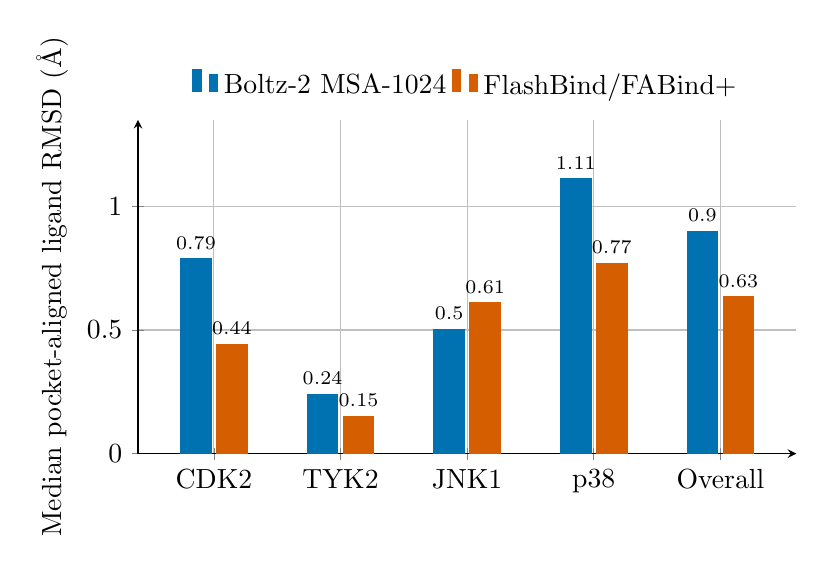
\begin{tikzpicture}
\begin{axis}[
  ybar,
  width=0.82\textwidth,
  height=0.48\textwidth,
  bar width=11pt,
  ymin=0,ymax=1.35,
  ylabel={Median pocket-aligned ligand RMSD (\AA)},
  xmin=-0.6,xmax=4.6,
  xtick={0,1,2,3,4},
  xticklabels={CDK2,TYK2,JNK1,p38,Overall},
  axis lines=left,
  grid=major,
  nodes near coords,
  nodes near coords style={font=\scriptsize},
  legend style={at={(0.5,1.03)},anchor=south,legend columns=2,draw=none},
]
\addplot[fill=cdk,draw=cdk] coordinates
  {(0,0.788) (1,0.238) (2,0.502) (3,1.111) (4,0.898)};
\addlegendentry{Boltz-2 MSA-1024}
\addplot[fill=tyk,draw=tyk] coordinates
  {(0,0.442) (1,0.150) (2,0.609) (3,0.768) (4,0.634)};
\addlegendentry{FlashBind/FABind+}
\end{axis}
\end{tikzpicture}
\caption{Median symmetry-corrected ligand RMSD by target and over all 16
structure-matched pairs. The target counts are CDK2 $n=6$, TYK2 $n=2$, JNK1
$n=1$, and p38 $n=7$; the JNK1 bar is therefore a single pair rather than a
stable target-level estimate. FlashBind has the lower overall median, but the
per-pair comparison remains mixed (9 lower for FlashBind and 7 for Boltz-2).}
\end{figure}

The released FlashBind/FABind+ poses were below 2~\AA{} for all 16 pairs,
whereas the Boltz-2 poses were below 2~\AA{} for 14. FlashBind had the lower
RMSD on 9 pairs and Boltz-2 on 7. The median paired FlashBind-minus-Boltz
difference was $-0.109$~\AA; its mean was $-0.326$~\AA, influenced by the two
Boltz poses above 2~\AA. This pattern does not support a claim of uniform
FlashBind superiority.

The protein decomposition changes the interpretation. Boltz-2's median global
protein C$\alpha$ RMSD was 1.231~\AA, while its median locally fitted pocket
C$\alpha$ RMSD was 0.400~\AA. The pocket result was strongly target-dependent:
the Boltz medians were 0.348~\AA{} for CDK2, 0.243~\AA{} for TYK2,
0.460~\AA{} for JNK1, and 2.305~\AA{} for p38. Thus the p38 ligand-pose result
coincides with a substantial local pocket-structure error and should not be
interpreted as ligand placement alone. In contrast, the FlashBind protein
pocket median was 0.208~\AA{} overall because it started from experimental PDB
protein structures.

I also audited the coordinate identities before scoring. Every released SDF
matched its reference ligand in heavy-atom count and admitted a complete
chemical graph mapping. The released p38 receptor has a formatting defect in
which the chain identifier disappears after residue 168; I joined the two
continuously numbered fragments in memory without changing coordinates and
recorded the repair. The archive documents these ligands as FABind+ docking
poses, but it does not contain the original docking commands, seeds, or
per-pose logs. Thus I have evaluated the supplied poses, not independently
reproduced their generation.

\section{Conclusion}

The three models address protein--ligand affinity in distinct ways. Boltz-2
uses protein sequence, ligand chemistry, and an MSA to generate an
atom-resolved complex and predict affinity. Nesso-1 predicts affinity from
protein sequence and ligand chemistry without generating a final Cartesian
complex. FlashBind instead scores a proposed three-dimensional complex; in
this benchmark, that complex consisted of an experimental PDB protein
structure and a FABind+-predicted ligand pose.

I reproduced the affinity-ranking result reported for each model on
the same 87-compound benchmark. The compound-weighted Pearson correlations
were 0.807 for Nesso-1, 0.627 for Boltz-2, and 0.533 for FlashBind, compared
with paper values of 0.80, 0.66, and 0.53, respectively. This close agreement shows
that the released models and the analysis used here reproduce the central
within-target ranking results from the three papers.

This agreement is a reproducibility result rather than an independent test of
generalization: all calculations use the same public benchmark, and the three
workflows do not receive equivalent structural information. It nevertheless
provides a validated starting point for studying how their architectures and
inputs produce affinity predictions.

\section{Next week's agenda}

Next week, I will move from reproducing benchmark results to understanding how
the three models produce those results. I will organize the architectures in
a common sequence---input representation, interaction module, structural or
pocket information, and affinity readout---so that their design choices can be
compared directly.

Using one protein--ligand pair as a worked example, I will trace the
information passed through each released implementation and address three
questions:
\begin{enumerate}
  \item How are the protein, ligand, MSA, and three-dimensional coordinates
  represented?
  \item How does each model combine protein and ligand information before the
  affinity head?
  \item Which controlled input changes can reveal what the prediction depends
  on, such as MSA depth for Boltz-2, protein-sequence changes for Nesso-1, and
  ligand-pose perturbations for FlashBind?
\end{enumerate}

The intended outputs are a common architecture diagram and a small notebook
that follows one example through the major stages of each model.

\section*{Technical methods}

Exact source revisions, checkpoint checksums, resolved inference settings,
commands, hardware records, output fields, and validation procedures are
documented separately in the
\href{https://github.com/Yusheng-cai/BindingAffinityPredictor/blob/main/weeks/2026-W34/technical-report/report.pdf}{Week 34 technical methods report}.
This presentation report retains only the procedural detail needed to
interpret the scientific comparisons.

\bibliographystyle{unsrtnat}
\bibliography{references}

\end{document}
